\documentclass[11pt,compress,t,notes=noshow, aspectratio=169, xcolor=table]{beamer}


\usepackage[nospeakermargin]{../../style/lmu-lecture-2}
% Defines macros and environments
\input{../../style/common.tex}
\usepackage{etoolbox}
\makeatletter
\newlength{\parboxtodim}
\patchcmd{\@iiiparbox}
  {\hsize}
  {\ifx\relax#2\else\setlength{\parboxtodim}{#2}\fi\hsize}
  {}{}
\makeatother
\begin{document}

\newcommand{\titlefigure}{figure/calibrationplot}
\newcommand{\learninggoals}{
\item What is calibration and discrimination?
\item Why or when are they important?
\item Standard approaches to diagnose whether a model is well-calibrated.}

\lecturechapter{Calibration versus Discrimination}
\lecture{Applied Machine Learning}

% scikitlearn calibration 
% https://scikit-learn.org/stable/modules/calibration.html

% \begin{frame}
%     \frametitle{Calibration Methods}
%     \framesubtitle{Introduction to Calibration}
    
%     \begin{itemize}
%         \item \textbf{Calibration:} The process of refining predicted probabilities to align with observed frequencies.
%         \item Necessary when model probabilities do not accurately reflect true probabilities.
%         \item Commonly used in classification tasks such as binary or multiclass classification.
%     \end{itemize}
% \end{frame}

% \begin{frame}
%     \frametitle{Platt Scaling}
    
%     Platt scaling is a logistic regression approach to calibrate predicted probabilities.
    
%     \begin{align*}
%         &\text{For binary classification:}\\
%         &\text{Model Output: } f(x) \\
%         &\text{Platt's Scaling: } P(y=1|x) = \frac{1}{1 + e^{a \cdot f(x) + b}}
%     \end{align*}
    
%     \begin{itemize}
%         \item Example: Logistic regression is trained on model predictions to estimate $a$ and $b$.
%     \end{itemize}
% \end{frame}

% \begin{frame}
%     \frametitle{Isotonic Regression}
    
%     Isotonic regression fits a non-decreasing function to calibrate predicted probabilities.
    
%     \begin{align*}
%         &\text{For binary classification:}\\
%         &\text{Model Output: } f(x) \\
%         &\text{Isotonic Regression: } P(y=1|x) = g(f(x))
%     \end{align*}
    
%     \begin{itemize}
%         \item Example: Piecewise constant function is fitted to map model predictions to calibrated probabilities.
%     \end{itemize}
% \end{frame}

% \begin{frame}
%     \frametitle{Beta Calibration}
    
%     Beta calibration is a method based on a parametric family of transformations.
    
%     \begin{align*}
%         &\text{For binary classification:}\\
%         &\text{Model Output: } f(x) \\
%         &\text{Beta Calibration: } P(y=1|x) = \frac{f(x)^{\alpha}}{f(x)^{\alpha} + (1 - f(x))^{\beta}}
%     \end{align*}
    
%     \begin{itemize}
%         \item Example: Parameters $\alpha$ and $\beta$ are learned through cross-validation or maximum likelihood estimation.
%     \end{itemize}
% \end{frame}

\begin{frame}{History of Calibration}
\begin{itemize}
    \item Weather forecasters began considering calibration in the 1950s. % (Brier, 1950).
    \item For all instances where a model predicts a '70\% chance of rain', it should actually have rained 70\% of the time (retrospectively).
    %\item Applicable to both binary and multi-class classification.
    \item In general, predicted probabilities for any event happening should (on average) match their observed empirical probabilities.\\
    $\Rightarrow$ Ensures predictions can be interpreted as actual risk/probabilities.
    %\item 
\end{itemize}
\end{frame}


\begin{frame}{Calibration and Discrimination}

Consider the true positive $Y=1$, true negative $Y=0$, and predicted label $\hat Y$.

\begin{itemize}
  \item<1-> \textbf{Discrimination:} Ability of $\hat Y$ to well-separate positive/negative instances.\\
  $\Rightarrow$ Confusion matrix-based measures are discrimination measures, e.g., $FPR = P(\hat Y = 1 | Y = 0$), $TPR = P(\hat Y = 1 | Y = 1)$, AUC.
  \item<1-> \textbf{Calibration:} When the predicted probabilities $\hat{p}$ closely agree with the observed proportion for $Y = 1$ (for any reasonable grouping).
  % \item Models can over-/underestimate probabilities (poor calibration) and still separate classes (good discrimination) or vice versa.
  % \item Poor calibration occurs with imbalanced classes or when the learner lacks a probabilistic framework (e.g., $k$-NN, trees).
  % \only<2-3> {\begin{itemize}
     \only<2-> {\item[$\Rightarrow$] \textbf{Calibration in the large:} %is a property of the \textit{full sample}.\\
      Observed vs. predicted prob. in \textit{full sample}.}
  %     
\includegraphics[page=3, width=0.85\textwidth]{figure_man/calibration_large_vs_small.pdf}}
     \visible<3> {\item[$\Rightarrow$] \textbf{Calibration in the small:} %is a property of \textit{subsets} of the sample.\\
     Observed vs. predicted prob. in \textit{subsets}.}
  %     
\includegraphics[page=4, width=0.85\textwidth]{figure_man/calibration_large_vs_small.pdf}}
  % \end{itemize}
  % }

  \only<2> {\centering
\includegraphics[page=3, width=0.75\textwidth]{figure_man/calibration_large_vs_small.pdf}}
  \only<3> {\centering
\includegraphics[page=4, width=0.75\textwidth]{figure_man/calibration_large_vs_small.pdf}}
\end{itemize}
\end{frame}



% \begin{frame}{Calibration versus Discrimination}

% \begin{itemize}
% \setlength\itemsep{1em}
%     \item Calibration indicates the agreement between estimated probabilities and observed class frequencies.
%     \item Discrimination is a model's ability to correctly separate observations into specific groups (depends on the selected threshold).
%     \item Models can over-/underestimate probabilities (poor calibration) and still separate classes (good discrimination) or vice versa.
%       \item Poor calibration occurs with imbalanced classes or when the learner lacks a probabilistic framework (e.g., $k$-NN, trees).
%   % \begin{itemize}
%   %   \item The learner has no probabilistic framework in the first place (e.g.,
%   %   $k$-NN or trees).
%   %   \item Classes are imbalanced.
%   % \end{itemize}
%   \item We distinguish between two different notions of calibration:
%   \begin{itemize}
%     \item \textbf{Calibration in the large} is a property of the 
%     \textit{full} sample.\\
%     $\rightarrow$ Observed class-1 frequency in full sample versus average overall predicted class-1 probability.
%     \item \textbf{Calibration in the small} is a property of \textit{subsets}.\\
%     $\rightarrow$ Observed likelihood in subset versus average predicted class-1 probability in that subset.
%   \end{itemize}
%     % \item Consider a model that predicts a patient's disease risk, where a patient is classified as a high-risk patient if disease risk exceeds 20\%. Patient A has a true risk of 5\% while patient B has a true risk of 30\%. The model predicts roughly the same risk with 19\% for A and 21\% for B. It is poorly calibrated but still separates both patients accurately into low-risk and high-risk groups (good discrimination).
    
% \end{itemize}

% \end{frame}

% \begin{frame}{Calibration in the Large}
%     % https://docs.google.com/presentation/d/1Drnq0Av_5KLfnwbRLnp-Tklgxc93C7BT_UXRCydtoes/edit#slide=id.p
    
%     %Compares observed probability (e.g. proportion of positive instances) with the average predicted probability in the \textit{full sample}.
%     
\includegraphics[page=3, width=0.6\textwidth]{figure_man/calibration_large_vs_small.pdf}
%     
\includegraphics[page=4, width=0.6\textwidth]{figure_man/calibration_large_vs_small.pdf}
% \end{frame}

% \begin{frame}{Calibration in the Small}
%     Compares observed proportion of positive instances  with the average predicted probability in each subset (often constructed by deciles).
%     \makebox[\linewidth]{\includegraphics[page=2, width=\textwidth]{figure/calibration_large_vs_small.pdf}}
% \end{frame}

% \begin{frame}{Why and When Is Calibration Important?}

%     \begin{itemize}
%         \item Reasoning / interpretation of predicted probabilities as actual risks.
%         \item If you are interested in the computed probability reflecting observed frequencies, you need good calibration.
%         %\item Assume a bank decides how much credit to grant to a customer.
%         %\item The bank needs a fairly accurate probability of default for each customer. The higher the default probability, the lower the loan.
%         %\item Given 1000 customers with a 40\% chance of default predicted by a well-calibrated model, we expect to see roughly 400 defaults in this customer group in our data set, etc.
%         %\item Accurate probabilities are necessary to ensure accurate forecasts of gains and losses of the bank.
%         %\item On the macroeconomic level, regulatory requirements demand accurate probabilities in bank models to ensure healthiness of the financial system as a whole.


%    \item \textbf{Example: Medical Diagnosis}

% \begin{itemize}
%     \item In medicine, a well-calibrated model is crucial for decision-making.
%     \item If a diagnostic test predicts 90\% probability of a disease, but only 50\% of patients with that predicted probability have the disease, it's poorly calibrated.
%     \item Poor calibration can lead to misdiagnosis, unnecessary medical procedures, or delayed treatment, impacting patient outcomes.
% \end{itemize}
%     \end{itemize}
% \end{frame}


% ------------------------------------------------------------------------------

% \begin{vbframe}{Discrimination}

% \begin{itemize}
%   \item Consider, again, the binary classification case.
%   \item \textbf{Discrimination} is the ability of a classifier to perfectly 
%   separate the population into positive and negative instances.
%   \begin{itemize}
%     \item The classifier is said to discriminate well if predictions differ 
%     strongly across classes -- e.g., predicted probabilities for the negative 
%     (positive) class are all close to zero (one).
%     \item Measures of discrimination: e.g., AUC, sensitivity, specificity.
%   \end{itemize}
% \end{itemize}

% \begin{center}
%   \includegraphics[width = 0.7\textwidth]{figure_man/placeholder_discrimination}
% \end{center}

% \end{vbframe}

% ------------------------------------------------------------------------------

% \begin{frame}{Calibration}

% \begin{itemize}
%   \item 
%   % \textbf{Calibration}, on the other hand, assesses the concordance of 
%   % predicted probabilities with the observed outcome (for any reasonable
%   % grouping). \\
%   For scoring classifiers, evaluating 
%   calibrations requires transformation of scores to posterior probabilities 
%   first.
%   \item Predictions of a well-calibrated classifier follow approximately the 
%   same distribution as the true data labels.
%   \item Poor calibration occurs with imbalanced classes or when the learner 
%   lacks a probabilistic framework (e.g., $k$-NN, trees).
%   % \begin{itemize}
%   %   \item The learner has no probabilistic framework in the first place (e.g.,
%   %   $k$-NN or trees).
%   %   \item Classes are imbalanced.
%   % \end{itemize}
%   \item We distinguish two different notions of calibration:
%   \begin{itemize}
%     \item \textbf{Calibration in the large} is a property of the 
%     \textit{full} sample.\\
%     $\rightarrow$ Observed class-1 frequency in full sample vs average overall 
%     predicted class-1 probability.
%     \item \textbf{Calibration in the small} is a property of \textit{subsets}.\\
%     $\rightarrow$ Observed likelihood in subset vs average predicted class-1 
%     probability in that subset.
%   \end{itemize}
% \end{itemize}

% We consider data with a binary outcome $y$.
% \begin{itemize}
%   \item \textbf{Calibration:} When the predicted probabilities closely agree
%     with the observed outcome (for any reasonable grouping).
%   \begin{itemize}
%     \item \textbf{Calibration in the large} is a property of the \textit{full sample}.
%     It compares the observed probability in the full sample  (e.g. proportion of observations for which $y=1$)
% <!-- (e.g., 10% if 10 of 100 individuals have the outcome being predicted, e.g. $y=1$) -->
%     with the average predicted probability in the full sample.
%     \item \textbf{Calibration in the small} is a property of \textit{subsets} of the sample.
%     It compares the observed probability in each subset with the average
%     predicted probability in that subset.
%   \end{itemize}
%   \item \textbf{Discrimination:} Ability to perfectly separate the population into $y=0$ and $y=1$.
%     Measures of discrimination are, for example, AUC, sensitivity, specificity.
% \end{itemize}

% \end{frame}

% ------------------------------------------------------------------------------

% \begin{frame}{Example}

% %<!-- http://www.uphs.upenn.edu/dgimhsr/documents/predictionrules.sp12.pdf -->
%  % \begin{table}[]
%  %    \scriptsize
%  %    \centering
%  %    \begin{tabular}{rrrrr}
%  %      \hline
%  %      ID & truth & prediction $f_1$ & prediction $f_2$ & prediction $f_3$ \\
%  %      \hline
%  %      1 & 1 & 0.9 & 0.6 & 0.9 \\
%  %      2 & 1 & 0.9 & 0.6 & 0.9 \\
%  %      3 & 1 & 0.9 & 0.4 & 0.9 \\
%  %      4 & 0 & 0.1 & 0.4 & 0.7 \\
%  %      5 & 0 & 0.1 & 0.4 & 0.7 \\
%  %      6 & 0 & 0.1 & 0.6 & 0.7 \\ \hline
%  %      avg. class-1 prob. & 50\%  & 50\%  & 50\% & 80\% \\
%  %      \hline
%  %    \end{tabular}
%  %  \end{table}
%  \begin{table}[]
%     \scriptsize
%     \centering
%     \begin{tabular}{rrrrr}
%       \hline
%       ID & truth & prediction $f_1$ & prediction $f_2$ \\
%       \hline
%       1 & 1 & 0.67 & 0.99  \\
%       2 & 1 & 0.67 & 0.99  \\
%       3 & 0 & 0.67 & 0.99  \\
%       4 & 1 & 0.33 & 0.01  \\
%       5 & 0 & 0.33 & 0.01  \\
%       6 & 0 & 0.33 & 0.01  \\

%       % avg. class-1 prob. & 50\%  & 50\%  & 50\% & 80\% \\
%       \hline
%     \end{tabular}
%   \end{table}


% \begin{itemize}
%   \item Classifier $f_1$ is both well-calibrated in the large and the small:
%     \begin{itemize}
%         \item For class-1-probabilities of 0.67, the observed relative freq. of class 1 is 0.67. The same holds for class-1-probabilities of 0.33. 
%         \item For a threshold of 0.5, its discriminative power, indicated by its accuracy, is 0.67.
%     \end{itemize}
%   \item Classifier $f_2$ is not well-calibrated but has the same discriminative power:
%     \begin{itemize}
%         \item For observations with class-1-probabilities of 0.99, one would expect a true label of class 1 almost every time.
%         \item Its discriminative power, with an accuracy of 0.67, is the same as for $f_1$.
%         \item $f_2$ is overconfident: its probabilities indicate that $f_2$ is too confident in classifying instances, which is not backed up by its accuracy.
%     \end{itemize}
%   % Both classifiers have identical calibration in the large, 
%   % but $f_1$ has better discriminative power.
%   % \lz
%   % \begin{table}[]
%   %   \centering
%   %   \begin{tabular}{rrrr}
%   %     \small
%   %     \hline
%   %     observation nr. & truth & prediction $f_1$ & prediction $f_2$ \\
%   %     \hline
%   %     1        & 1     & 1           & 0           \\
%   %     2        & 1     & 1           & 1           \\
%   %     3        & 0     & 0           & 1           \\
%   %     4        & 0     & 0           & 0           \\ \hline
%   %     avg. class-1 prob. & 50\%  & 50\%        & 50\%        \\
%   %     \hline
%   %   \end{tabular}
%   % \end{table}

%   % \lz
% % <<eval = FALSE, echo = FALSE>>=
% % truth = c(1,1,0,0,0,0)
% % pred.rule.1 = c(1,1,0,0,0,0)
% % pred.rule.2 = c(0,0,0,0,1,1)
% % kable(data.frame(truth = truth, "pred rule 1" = pred.rule.1, "pred rule 2" = pred.rule.2))
% % @
% % \lz
% %   \item Conversely, $f_1$ and $f_3$ both discriminate well (e.g., setting thresholds at
% %   0.5 and 0.8, respectively), but $f_3$ is poorly calibrated with class 1 being estimated at an 80\% frequency, as opposed to a true frequency of 50\%.
% %   % \lz
%   %   \begin{table}[]
%   %   \footnotesize
%   %   % \centering
%   %   \begin{tabular}{rrrr}
%   %     \hline
%   %     observation nr. & truth & prediction $f_1$ & prediction $f_2$ \\
%   %     \hline
%   %     1 & 1 & 0.97 & 0.66 \\
%   %     2 & 1 & 0.97 & 0.66 \\
%   %     3 & 0 & 0.01 & 0.45 \\
%   %     4 & 0 & 0.01 & 0.45 \\
%   %     5 & 0 & 0.01 & 0.45 \\
%   %     6 & 0 & 0.01 & 0.45 \\
%   %     % 7 & 0 & 0.01 & 0.67 \\
%   %     % 8 & 0 & 0.01 & 0.67 \\ \hline
%   %     avg. class-1 prob. & 25\%  & 25\%  & 75\% \\
%   %     \hline
%   %   \end{tabular}
%   % \end{table}
%   % \begin{table}[]
%   %   \footnotesize
%   %   % \centering
%   %   \begin{tabular}{rrrr}
%   %     \hline
%   %     observation nr. & truth & prediction $f_1$ & prediction $f_2$ \\
%   %     \hline
%   %     1 & 1 & 0.97 & 0.99 \\
%   %     2 & 1 & 0.97 & 0.99 \\
%   %     3 & 0 & 0.01 & 0.67 \\
%   %     4 & 0 & 0.01 & 0.67 \\
%   %     5 & 0 & 0.01 & 0.67 \\
%   %     6 & 0 & 0.01 & 0.67 \\
%   %     7 & 0 & 0.01 & 0.67 \\
%   %     8 & 0 & 0.01 & 0.67 \\ \hline
%   %     avg. class-1 prob. & 25\%  & 25\%  & 75\% \\
%   %     \hline
%   %   \end{tabular}
%   % \end{table}
%   % \begin{table}[]
%   %  \scriptsize
%   % \centering
%   % \begin{tabular}{rrrr}

%   % \hline
%   % observation nr. & truth & prediction $f_1$ & prediction $f_2$ \\
%   % \hline
%   % 1        & 1     & 0.9           & 0.9         \\
%   % 2        & 1     & 0.9           & 0.9           \\
%   % 3        & 0     & 0.1          & 0.7           \\
%   % 4        & 0     & 0.1         & 0.7           \\ \hline
%   % avg. class-1 prob. & 50\%  & 50\%        & 80\%        \\
%   % \hline
%   % \end{tabular}
%   % \end{table}
%   % \lz
%   % \item Both classifiers discriminate well (e.g., setting thresholds at
%   % 0.5 and 0.8, respectively).
%   % \item Classifier $f_2$ is, however, rather poorly calibrated: the probability 
%   % of class 1 would be estimated at three times the true proportion.
% \end{itemize}
% \end{frame}




\begin{frame}{Calibration and Discrimination}
%<!-- http://www.uphs.upenn.edu/dgimhsr/documents/predictionrules.sp12.pdf -->
A well calibrated classifier can be poorly discriminating, e.g.

\begin{table}[]
\centering
\begin{tabular}{r|rrr}
\hline
Obs. Nr. & true $Y$ & $\fh_1$ & $\fh_2$ \\
\hline
1        & 1     & 1           & 0           \\
2        & 1     & 1           & 0           \\
3        & 0     & 0           & 1           \\
4        & 0     & 0           & 1           \\ \hline
Avg Prob & 50\%  & 50\%        & 50\%        \\
\hline
\end{tabular}
\end{table}

\begin{itemize}
  \item Both models ($\fh_1$ and $\fh_2$) result in the same calibration in the large (50\%).
  \item However, $\fh_1$ is better than $\fh_2$ as it correctly classifies the real outcome $Y$.
\end{itemize}

\end{frame}

\begin{frame}{Calibration and Discrimination}
A well discriminating classifier can have a bad calibration, e.g.

\begin{table}[]
\centering
\begin{tabular}{rrrr}
\hline
Obs. Nr. & truth $Y$ & $\fh_1$ & $\fh_2$ \\
\hline
1        & 1     & 0.9           & 0.9         \\
2        & 1     & 0.9           & 0.9           \\
3        & 0     & 0.1          & 0.7           \\
4        & 0     & 0.1         & 0.7           \\ \hline
Avg Prob & 50\%  & 50\%        & 80\%        \\
\hline
\end{tabular}
\end{table}

\begin{itemize}
  \item Both models are well discriminating, i.e., setting thresholds $c_1 = 0.5$ for $\fh_1$ and $c_2 = 0.8$ for $\fh_2$ perfectly separates positive and negative observations (and will result, e.g., in the same AUC).
  \item $\fh_2$ is poorly calibrated as the averaged probabilities are $80\%$ and do not match the truth proportion of positive observations (which is $50\%$).
\end{itemize}

\end{frame}

% \begin{frame}{Importance of Calibration}

% % \textbf{Example 1: Weather Forecasting}

% % \begin{itemize}
% %     \item Consider a weather forecasting model that predicts the probability of rain.
% %     \item If the model consistently predicts a 70\% chance of rain, but it actually rains only 10\% of the time when it predicts a 70\% chance, it's poorly calibrated.
% %     \item Poor calibration can lead to bad decisions (carrying an umbrella unnecessarily).
% % \end{itemize}

% \textbf{Example: Medical Diagnosis}

% \begin{itemize}
%     \item In medicine, a well-calibrated model is crucial for decision-making.
%     \item If a diagnostic test predicts 90\% probability of a disease, but only 50\% of patients with that predicted probability have the disease, it's poorly calibrated.
%     \item Poor calibration can lead to misdiagnosis, unnecessary medical procedures, or delayed treatment, impacting patient outcomes.
% \end{itemize}

% \end{frame}





\begin{frame}{Over- and Under-estimates}

Consider the following predictions of a (good performing) classifier:

\begin{columns}[c, onlytextwidth]
    \begin{column}{0.3\textwidth}
        \begin{center}
\begin{tabular}{rrr}
\hline
 & $\hat{p}$ & $y$ \\
\hline
0 & 0.1 & 0 \\
1 & 0.1 & 0 \\
\hline
2 & 0.4 & 0 \\
3 & 0.4 & 1 \\
\hline
4 & 0.7 & 0 \\
5 & 0.7 & 1 \\
6 & 0.7 & 1 \\
\hline
7 & 0.9 & 1 \\
\hline
\end{tabular}
\end{center}
    \end{column}
        \begin{column}{0.7\textwidth}
\begin{itemize}
    \item '10\% chance of rain' was a slight over-estimate ($\bar{y}=0/2=0\%$).
    \item '40\% chance of rain' was a slight under-estimate ($\bar{y}=1/2=50\%$).
    \item '70\% chance of rain' was a slight over-estimate ($\bar{y}=2/3=67\%$).
    \item '90\% chance of rain' was a slight under-estimate ($\bar{y}=1/1=100\%$).
\end{itemize}
    \end{column}
\end{columns}
%\vspace{1em}
%\textbf{Calibration}: Is a post-processing step on predicted probabilities trying to reduce over- and under-estimates.
\end{frame}





\begin{frame}{Calibration Plot / Reliability Diagram}

%\fbox{
\parbox[][45pt][t]{\linewidth}{%
 To detect calibration, we can visualize on the
\begin{itemize}
    \item $x$-axis: average predicted probability (e.g., grouped by quantiles) 
    \item $y$-axis: observed proportion of positive instances in each group
\end{itemize}
}
%}

\begin{columns}[c, onlytextwidth]
    \begin{column}{0.3\textwidth}
\begin{center}
\begin{tabular}{rrr}
\hline
 & $\hat{p}$ & $y$ \\
\hline
0 & 0.1 & 0 \\
1 & 0.1 & 0 \\
\hline
2 & 0.4 & 0 \\
3 & 0.4 & 1 \\
\hline
4 & 0.7 & 0 \\
5 & 0.7 & 1 \\
6 & 0.7 & 1 \\
\hline
7 & 0.9 & 1 \\
\hline
\end{tabular}
\end{center}
 \end{column}
        \begin{column}{0.7\textwidth}
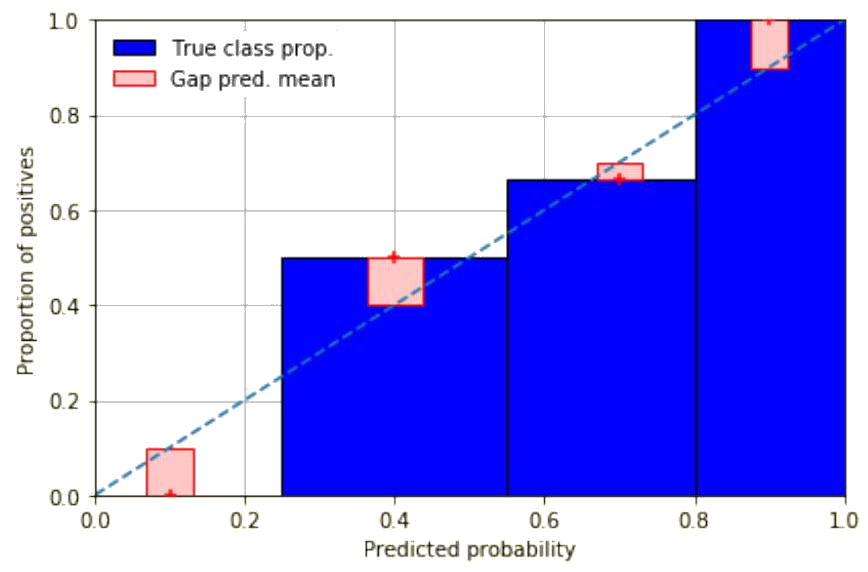
\includegraphics[width=\textwidth]{figure_man/calibplot}

    \end{column}
\end{columns}


\end{frame}



\begin{frame}{Calibration Plot / Reliability Diagram}

\parbox[][45pt][t]{\linewidth}{%
Changing predictions will change the position of the red points on the x-axis
\begin{itemize}
    \item[$\Rightarrow$] The closer the points to the diagonal line, the better calibration
    \item[$\Rightarrow$] \textit{Gap pred. mean} shows deviation between points and diagonal line
\end{itemize}
}

\begin{columns}[c, onlytextwidth]
    \begin{column}{0.3\textwidth}


\begin{center}
\begin{tabular}{rrr}
\hline
 & $\hat{p}$ & $y$ \\
\hline
0 & 0.1 & 0 \\
1 & \textbf{0.2} & 0 \\
\hline
2 & \textbf{0.3} & 0 \\
3 & 0.4 & 1 \\
\hline
4 & \textbf{0.6} & 0 \\
5 & 0.7 & 1 \\
6 & \textbf{0.8} & 1 \\
\hline
7 & 0.9 & 1 \\
\hline
\end{tabular}
\end{center}

 \end{column}
        \begin{column}{0.7\textwidth}
\begin{center}
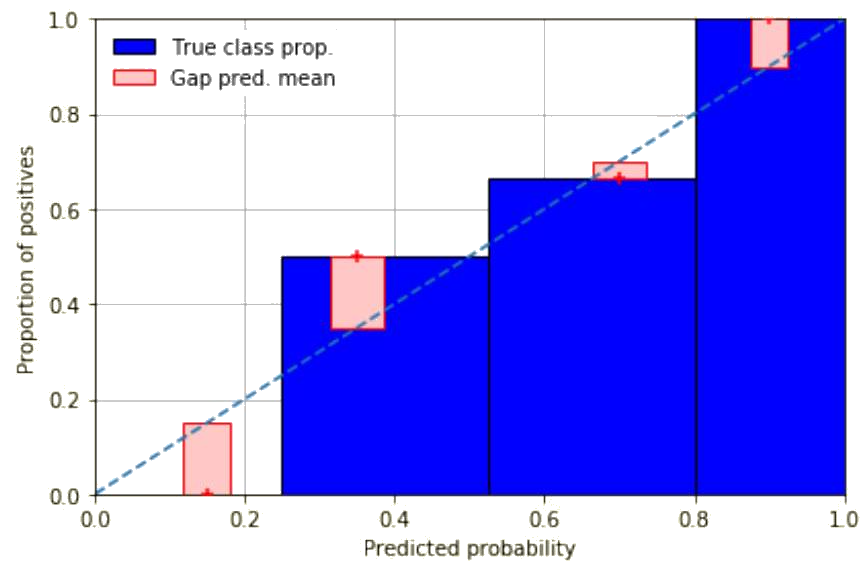
\includegraphics[width=\textwidth]{figure_man/calibplot-2}
\end{center}

    \end{column}
\end{columns}

\textbf{Question:} Did we improve or worsen calibration?
\end{frame}




% Frame: Or should we group forecasts differently?
\begin{frame}{Calibration Plot / Reliability Diagram}


Different groupings lead to a completely different picture

\begin{center}
    
\begin{columns}[c, onlytextwidth]
    \begin{column}{0.35\textwidth}

\footnotesize
\raggedleft
\begin{tabular}{rrr}
\hline
 & $\hat{p}$ & $y$ \\
\hline
0 & 0.1 & 0 \\
1 & 0.2 & 0 \\
2 & 0.3 & 0 \\
3 & 0.4 & 1 \\
\hline
4 & 0.6 & 0 \\
5 & 0.7 & 1 \\
6 & 0.8 & 1 \\
7 & 0.9 & 1 \\
\hline
\end{tabular}

 \end{column}
        \begin{column}{0.5\textwidth}
        \raggedright
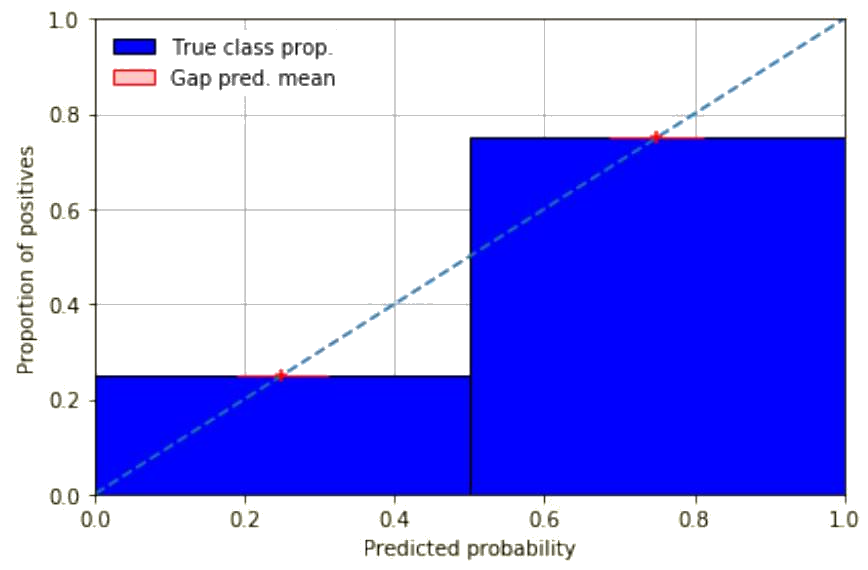
\includegraphics[width=0.9\textwidth]{figure_man/calibplot-3}

    \end{column}
    \begin{column}{0.15\textwidth}
    \end{column}
\end{columns}

\begin{columns}[c, onlytextwidth]
    \begin{column}{0.35\textwidth}
\footnotesize
\raggedleft
\begin{tabular}{rrr}
\hline
 & $\hat{p}$ & $y$ \\
\hline
0 & 0.1 & 0 \\
\hline
1 & 0.2 & 0 \\
\hline
2 & 0.3 & 0 \\
\hline
3 & 0.4 & 1 \\
\hline
4 & 0.6 & 0 \\
\hline
5 & 0.7 & 1 \\
\hline
6 & 0.8 & 1 \\
\hline
7 & 0.9 & 1 \\
\hline
\end{tabular}

 \end{column}
        \begin{column}{0.5\textwidth}
        \raggedright
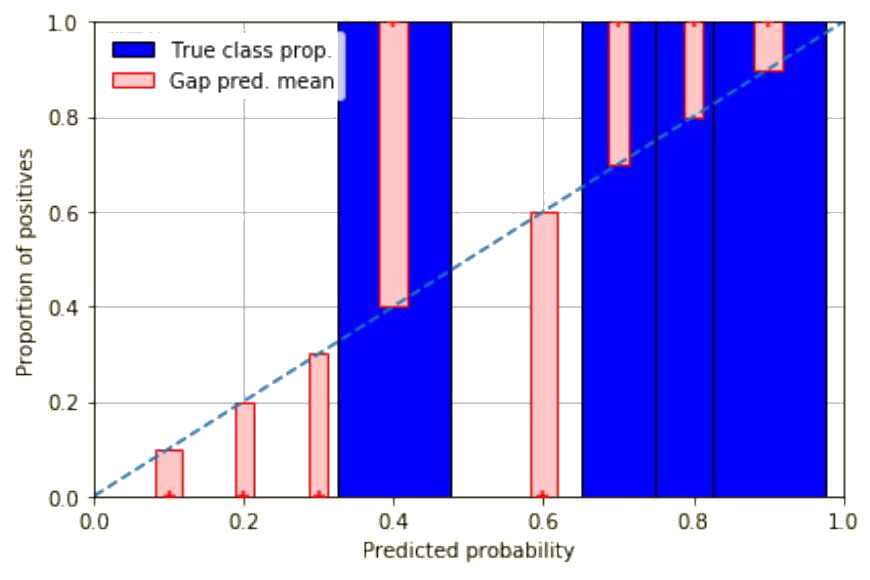
\includegraphics[width=0.9\textwidth]{figure_man/calibplot-4}

    \end{column}    
    \begin{column}{0.15\textwidth}
    \end{column}
\end{columns}

\end{center}
\end{frame}

% Frame: Binning or pooling predictions is a fundamental notion
\begin{frame}{Importance of grouping predictions}
\textbf{Evaluating calibration with bins/groups:}
\begin{itemize}
    \item We need a sufficient number of predictions within each group to obtain reliable empirical estimates.
    \item Trade-off: large groups give better empirical estimates, small groups allow a more fine-grained assessment of calibration.
\end{itemize}
% But adjusting forecasts in groups also gives rise to practical calibration methods:
% \begin{itemize}
%     \item empirical binning
%     \item isotonic regression (aka ROC convex hull)
% \end{itemize}
\pause 
\textbf{How groups/bins can be created:}
\begin{itemize}
\item Equal-Width: Splits predicted probabilities into equally sized intervals.\\
$\Rightarrow$ Can lead to bins with few or no observations.
\item Equal-Frequency: Each bin holds a similar number of observations.\\
$\Rightarrow$ Bin width can vary notably; Issues with duplicated values.
% \item Empirical Binning: Uses unique values to create bins containing at least a desired number of observations.\\
% $\Rightarrow$ Bin width and bin size may vary; Useful with duplicated values.% similar to equal-frequency in case of no duplicates.
\end{itemize}
\end{frame}




\begin{frame}{ROC Curve vs. Calibration Plot}

{\centering 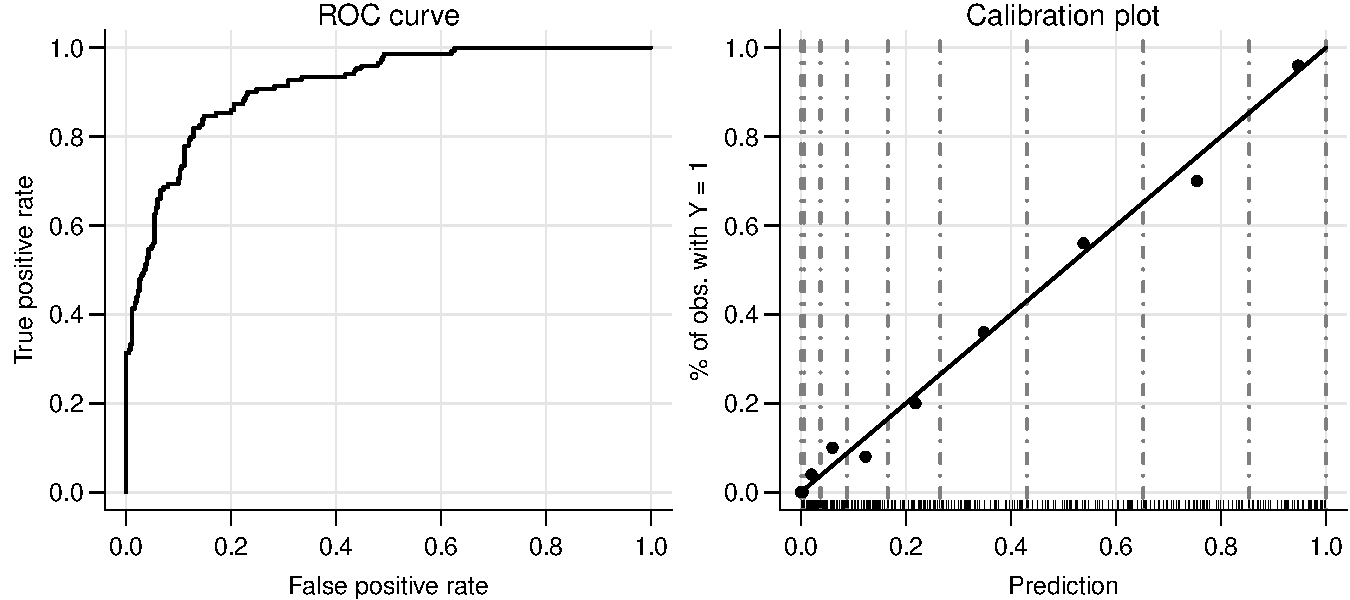
\includegraphics[width=\textwidth]{figure_man/calibdiscr1}}

% and do not visualize how well-calibrated the probabilities are.
%To assess the performance of classifiers, we should consider:
\begin{itemize}
\item \textbf{ROC:}
Measures only discrimination as it is based on TPR and FPR and assesses only the ranking of predicted probabilities (not their magnitude).
%Measures the ability to separate the classes well. % (e.g., confusion matrix). %accurately rank individuals from low to high risk.
\item \textbf{Calibration plot:} Measures (for reasonable groupings) how well the predicted probabilities match the proportion of positives. %(i.e., $Y = 1$).
\end{itemize}

\end{frame}



\begin{frame}{ROC Curve vs. Calibration Plot}

{\centering 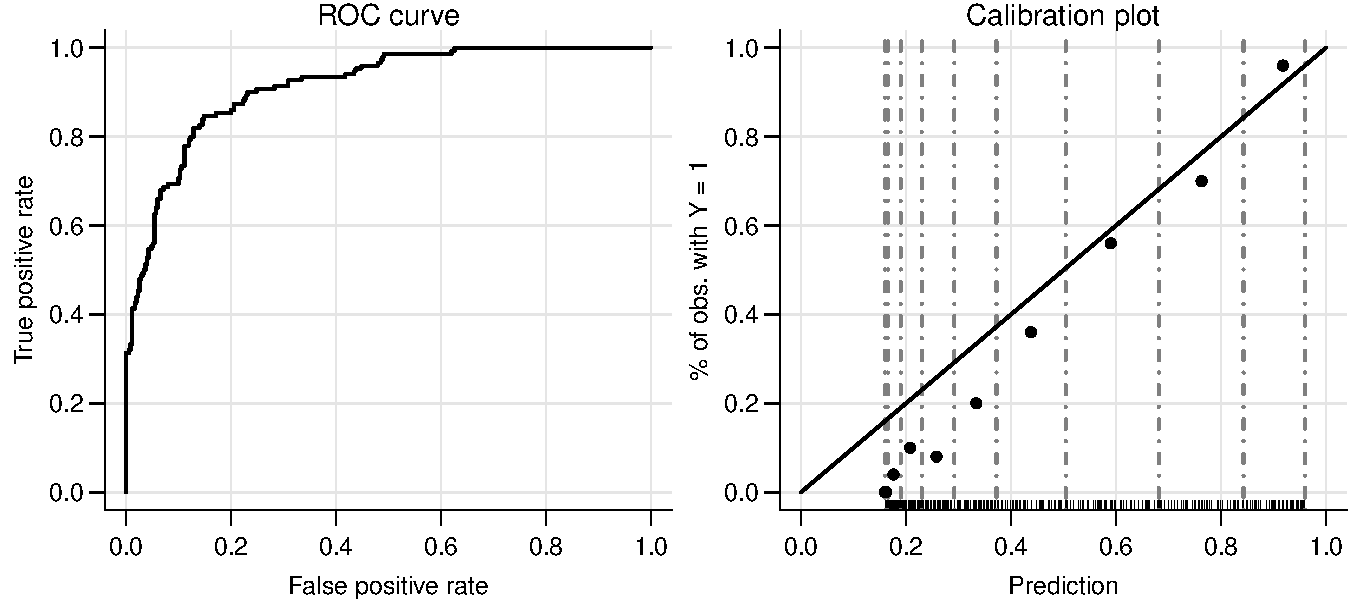
\includegraphics[width=\textwidth]{figure_man/calibdiscr3}}

\vspace{0.5em}

Monotonic transformations of the predicted probabilities (e.g., $\tfrac{\hat p + 0.2}{1.2}$)
\begin{itemize}
\item do not affect the ROC curve as the ranking will not change.
\item affect the calibration plot (here it looks worse). %as the probabilities are changed.
\end{itemize}
\end{frame}


\begin{frame}{ROC Curve vs. Calibration Plot}

{\centering 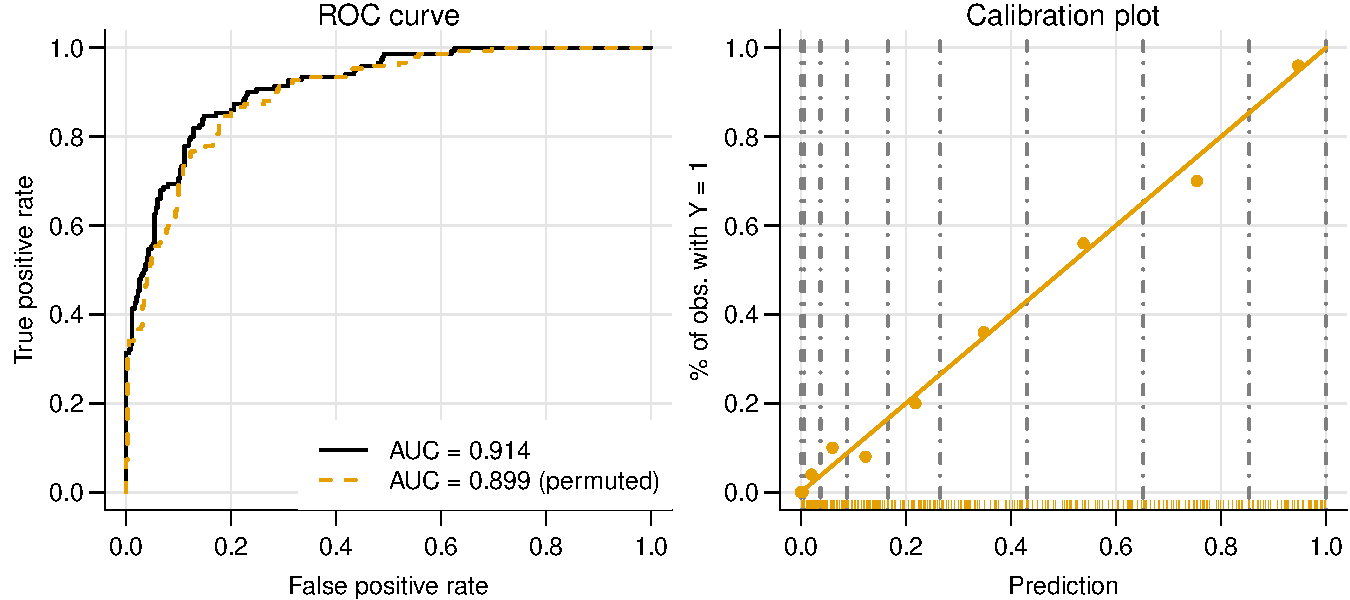
\includegraphics[width=\textwidth]{figure_man/calibdiscr2}}

\vspace{0.5em}

Permuting the predictions (e.g., randomly assigning different predictions to observations) within each decile 

\begin{itemize}
\item worsens the ROC curve /  AUC (ranking within each decile changes).
\item does not affect the calibration plot.
\end{itemize}


\end{frame}






% \begin{frame}{Calibration Plots}

% \begin{columns}[c, onlytextwidth]
%     \begin{column}{0.61\linewidth}
% 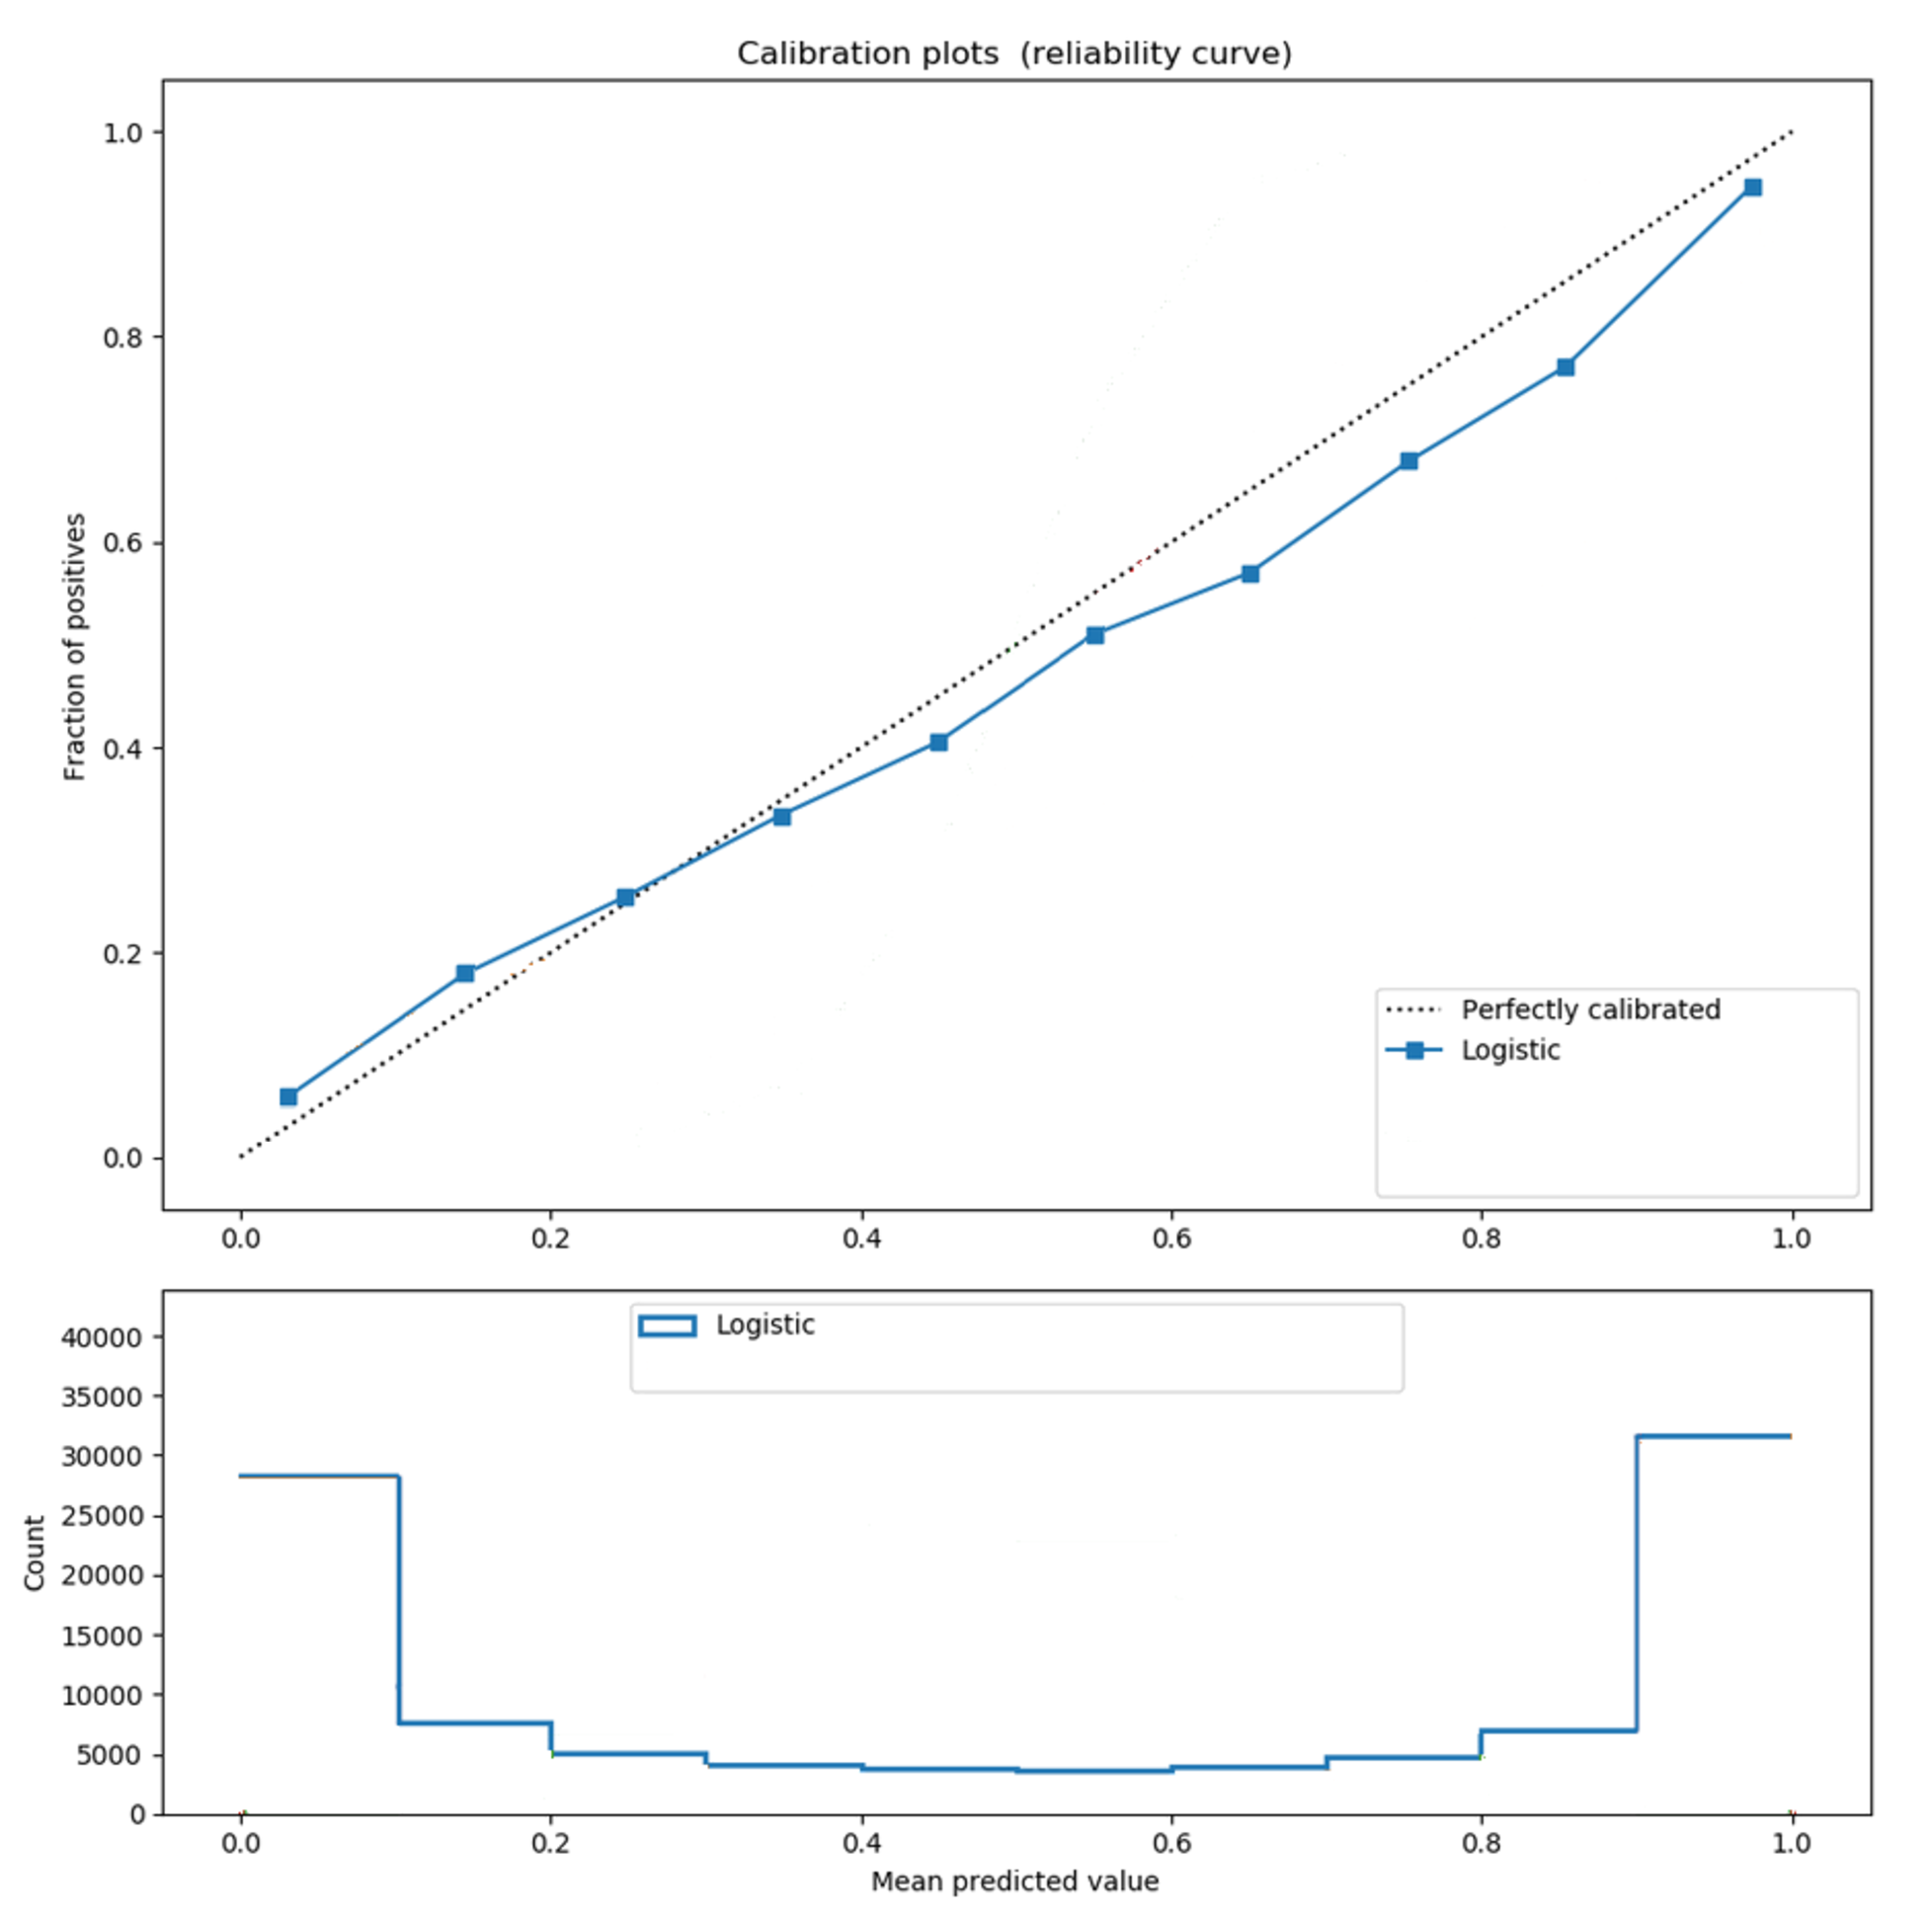
\includegraphics[width=\textwidth, page=1]{figure_man/calibration.pdf}
%     \end{column}
%       \begin{column}{0.39\linewidth}
        
% Calibration plots (reliability diagrams) visualize on
% \begin{itemize}
%     \item $x$-axis: average predicted probability (e.g., grouped by quantiles) 
%     \item $y$-axis: observed proportion of positive instances in each group
% \end{itemize}

%     \end{column}
% \end{columns}

%\end{frame}

\begin{frame}{Example: Calibration Plots}


\begin{columns}[c, onlytextwidth]
    \begin{column}{0.61\linewidth}

\only<1>{
\includegraphics[width=\textwidth, page=2]{figure_man/calibration.pdf}}
\only<2>{\includegraphics[width=\textwidth, page=3]{figure_man/calibration.pdf}}
\only<3>{\includegraphics[width=\textwidth, page=4]{figure_man/calibration.pdf}}

    \end{column}
      \begin{column}{0.39\linewidth}

        

\begin{itemize}
 %\item Logistic regression is already well-calibrated as it optimzes log-loss
 \item<1-> Many algorithms (except logistic regression) return biased probabilities.
 \item<1-> Linear SVC: badly calibrated, as predictions refer to a distance to decision boundary and not to probabilities.
 \item<2-> Random Forest: probabilities close to 0 or 1 are very rare.
 \item<3-> Naive Bayes: pushes probabilities to 0 or 1 (see histograms).
 %Base-level trees trained with random forests incorporate relatively high variance due to feature subsisting
 %(Niculescu-Mizil and Caruana 2005).

\end{itemize}
    \end{column}
\end{columns}

\end{frame}


\begin{frame}{Calibrating Probabilities}

\begin{itemize}
  \item Calibrating probabilities means to post-process the predictions to improve the estimates and obtain more reliable probabilities.
  %\item Two popular calibration methods are the \textbf{Platt’s scaling} (parametric) and the \textbf{isotonic regression} (non-parametric).
  \item A well calibrated classifier should classify samples such that among these samples with a predicted probability of 0.7, approximately 70\% actually belong to the positive class.
  \item The link function of logistic regression is basically a calibration for the scores predicted by linear regression.
  \item Note that calibration should be performed on new data not used for model fitting.
\end{itemize}

%In order to extract exact probabilities, like logarithmic loss does, a classifier can be calibrated, i.\,e. the output score of the calssifier can be transformed into a more accurate probability. The link function of logisitc regression is basically a calibration for the linear regression. In order to evaluate the calibration an additional validation data set is used. \lz
\end{frame}


\begin{frame}{Calibrating Probabilities}

The \textbf{Platt's scaling} (parametric sigmoid calibration) and the \textbf{isotonic regression} (non-parametric) are popular calibration methods:
\begin{itemize}
\item \textbf{Platt's scaling:} logistic regression on the output of the classifier with respect to the true class labels.
\item \textbf{Isotonic regression:} fit a piecewise-constant non-decreasing function instead of logistic regression.
\end{itemize}

%\tiny{Source 1: https://scikit-learn.org/stable/modules/calibration.html}
%\tiny{Source 2: http://fastml.com/classifier-calibration-with-platts-scaling-and-isotonic-regression/}
%\tiny{Source 3: https://towardsdatascience.com/probability-calibration-for-boosted-trees-24cbd0f0ccae}
%\tiny{Source 3: https://jmetzen.github.io/2015-04-14/calibration.html}
%\tiny{Source 4: http://fa.bianp.net/blog/2013/isotonic-regression/}
%\tiny{Source 5: https://www.analyticsvidhya.com/blog/2016/07/platt-scaling-isotonic-regression-minimize-logloss-error/}


\textbf{Platt's scaling}:

\begin{itemize}
  \item Train a logistic regression model using the (uncalibrated) classifier's predictions $\hat{Y}$ as input and the true labels as output.
  \item Use the probabilities $\hat{\pi}$ of this logistic regression model as calibrated predictions.
  %\item Essentially Platt's scaling performs a logistic regression on the output of a classifier.
\end{itemize}
% \begin{center}
% \includegraphics[width=0.55\textwidth]{figure_man/platt.png}
% \end{center}


\end{frame}


\begin{frame}{Platt's Scaling}

\begin{figure}
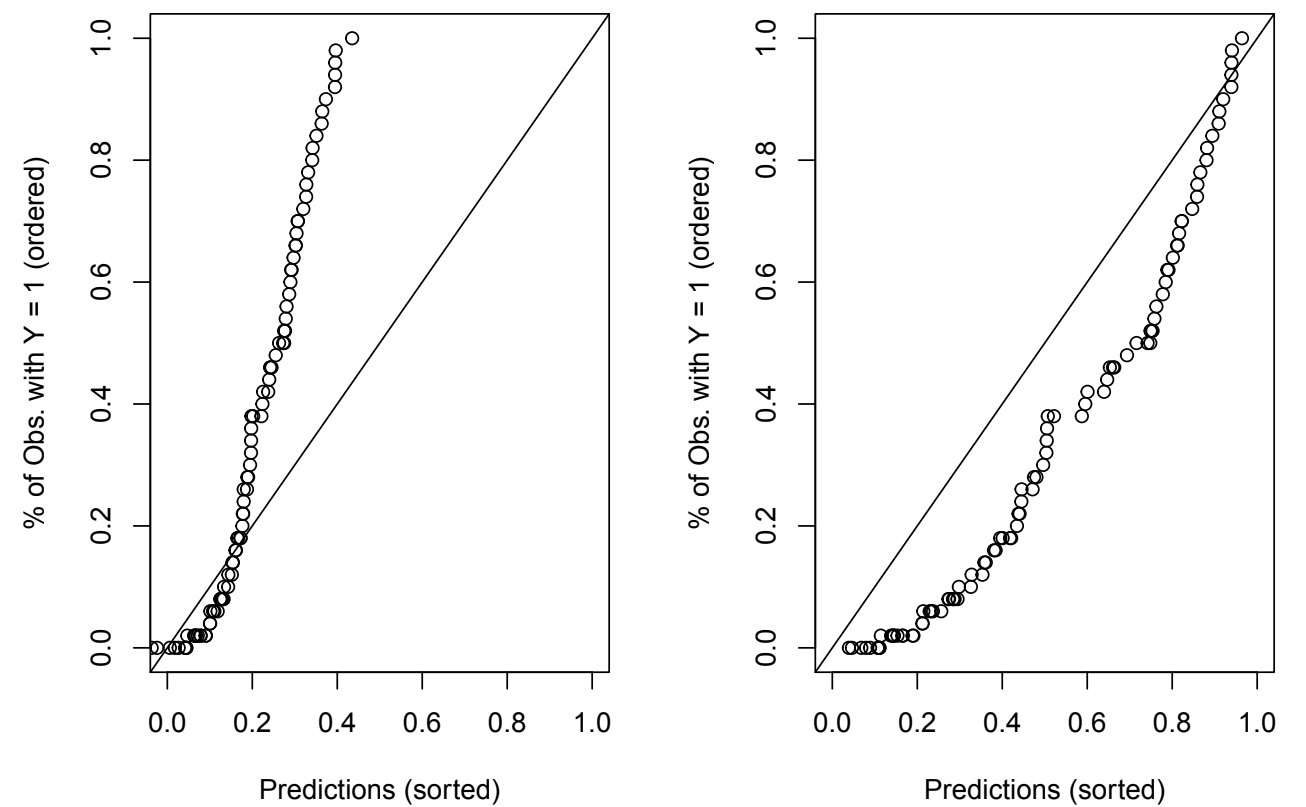
\includegraphics[width=0.8\textwidth]{figure_man/platts-scaling.png}
\end{figure}

\end{frame}


\begin{frame}{Isotonic regression}

\begin{itemize}
\item The idea is to fit a piecewise-constant non-decreasing function instead of
logistic regression with the pool adjacent violators algorithm
($\mathcal{O}(n)$).
\item Basically, the algorithm goes through the data and looks for violations of
the monotonicity constraint. If it finds one, it gets adjusted with the best
possible fit under the constraint.
\end{itemize}

\begin{center}
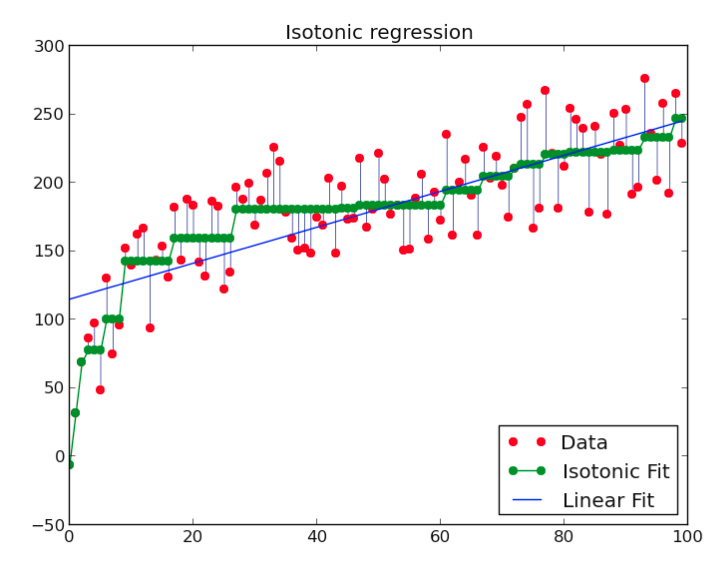
\includegraphics[width=0.5\textwidth]{figure_man/iso-reg.png}
\end{center}
\end{frame}
\begin{frame}{Isotonic regression}

\begin{figure}
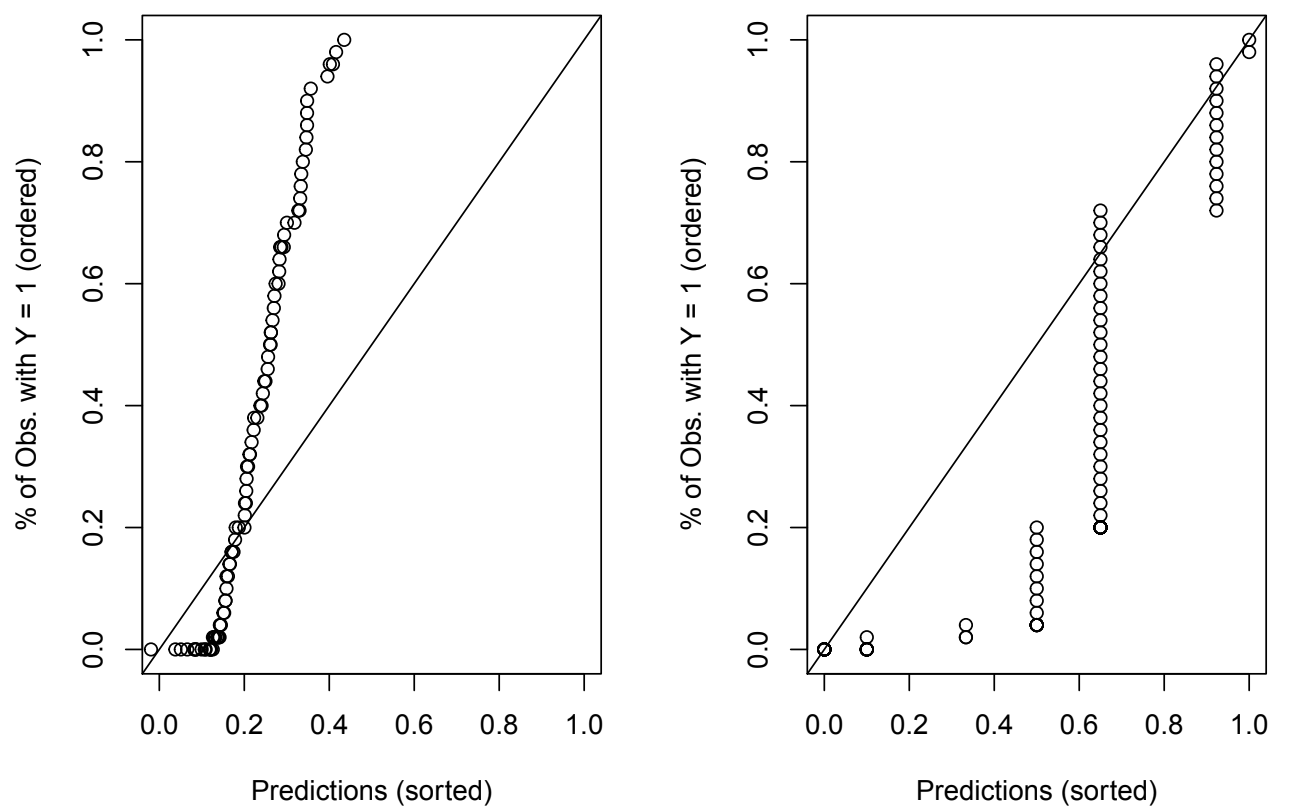
\includegraphics[width=0.8\textwidth]{figure_man/isotonic-reg.png}
\end{figure}

\end{frame}


\begin{frame}{Example: Calibration Plot}

Calibrating a SVC with Platt's scaling and isotonic regression:
\begin{center}
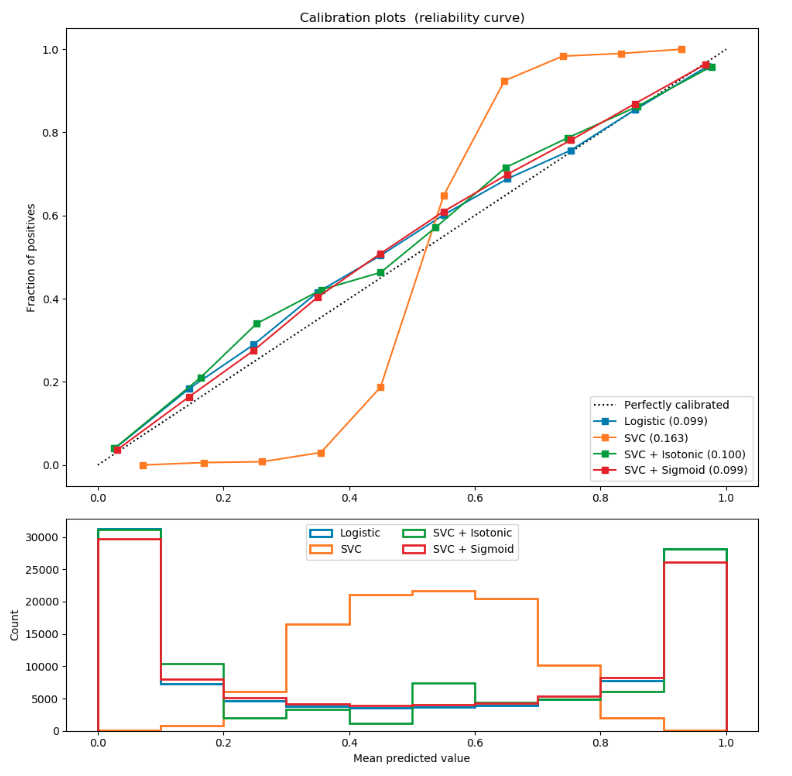
\includegraphics[width=0.6\textwidth]{figure_man/calibration2.png}
\end{center}

\end{frame}




% \begin{frame}{Diagnosis with Reliability Diagrams}
%     % https://www.cs.cornell.edu/~alexn/papers/calibration.icml05.crc.rev3.pdf
%     To Do: selbst coden
%     \begin{figure}
%         \centering
%         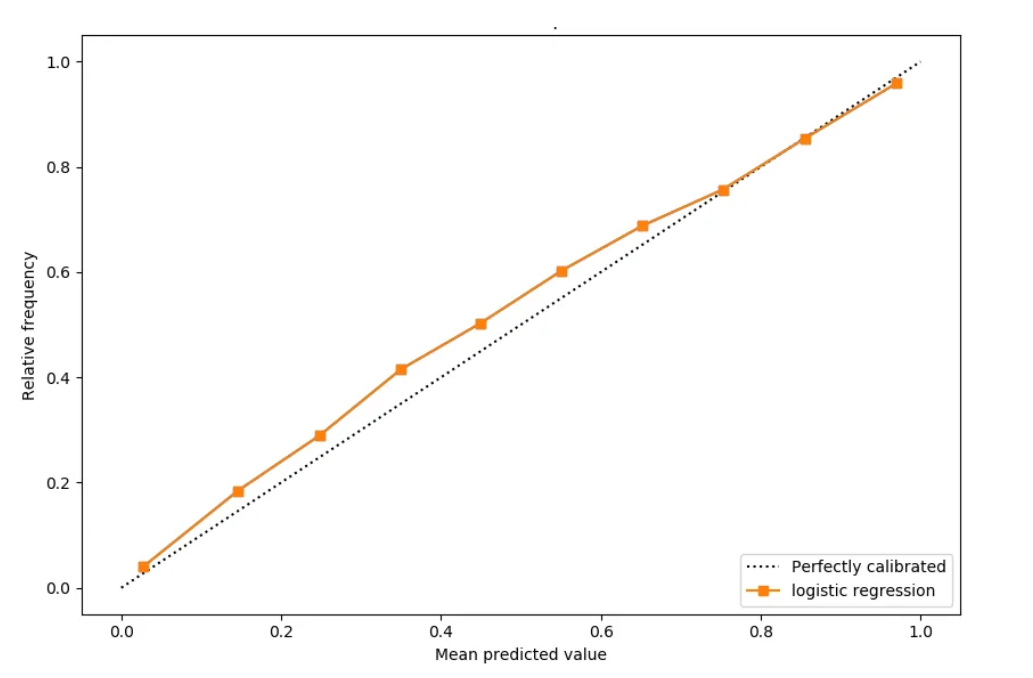
\includegraphics{figure/reliability_diagram.png}
%         % \caption{Caption}
%         % \label{fig:enter-label}
%     \end{figure}
% \end{frame}

% --------------------------------------

\begin{frame}{Sources of Miscalibration}
% https://classifier-calibration.github.io/assets/slides/clacal_tutorial_ecmlpkdd_2020_intro.pdf
\begin{itemize}
    \item Calibration is a characteristic of a learner, e.g., tree-based learners such as CART or random forests seldom produce probabilities close to 0 or 1 due to averaging class values. 
    \item Miscalibration is related to accuracy: if the average class probability is higher or lower than accuracy, the model is said to be over- or underconfident.
    \item \textbf{Underconfidence:} Probabilities are underestimating true incidences. This typically gives a sigmoidal reliability diagram.
    $\Rightarrow$ We need to pull probabilities away from the center.
    \item \textbf{Overconfidence:} Probabilities are overestimating true incidences.  This typically gives an inverse-sigmoidal reliability diagram. $\Rightarrow$ We need to push probabilities toward the center.
    \item \textbf{Predicament:} Under- and overconfidence can coexist for different classes, requiring a simultaneous increase and decrease in different class probabilities.

\end{itemize}
\end{frame}

\begin{frame}[t]
	\frametitle{How To Do Calibration}
	\small
	\begin{itemize}
% %		
% 		\item Consider binary classification with a probabilistic score  classifier
% %		
% 		$$\fx = 2 \cdot \mathds{1}_{[ s(\xv) \ge c]} -1,$$
% %		
% 		leading to the prediction random variable $\yh = f(\xv).$ Let $\mathbf{S}=s(\xv)$ be the score random variable. 
% %		
% 		\item $f$ is calibrated iff $P(y=1~|~\mathbf{S}=s) = s$ for all $s\in [0,1].$
%		
		\item Let $s(\xv)$ be the predicted (uncalibrated) score/probability of instance $\xv$ and $\mathbb{S}$ the set of possible scores produced by the classifier.
        \item Different \emph{post-processing} methods have been proposed for the purpose of calibration, i.e., to construct a \emph{calibration function} 
%		
		$$C: \, \mathbb{S} \to [0,1], $$
		such that $C(s(\xv))$ is well-calibrated.
		
		\item For learning a calibration function $C$, a set of \emph{calibration data} is used:
		$$
		\mathcal{D}_{cal} = \big\{ (s^{(1)}, y^{(1)}) , \ldots , (s^{(n)}, y^{(n)}) \big\} \subset \mathbb{S} \times \{ 0 , 1 \}
		$$ 
		
		\item This data should be different from the training data used to learn the scoring classifier. Otherwise, there is a risk of introducing a bias. 
		
	\end{itemize}
\end{frame}

\begin{frame}[t]
	\frametitle{Empirical binning}
	% https://link.springer.com/article/10.1007/s10994-023-06336-7
	\begin{itemize}
		\item \emph{Empirical binning} partitions the scores \( s \in \mathbb{S}\) into bins \( B_1, \ldots, B_M \) and defines a (piecewise constant) calibration function \( C \) by:

\[ 
C(s) = \bar{p}_{J(s)} = \frac{\sum_{i=1}^n \mathds{1}[s(\xi) \in B_{J(s)}] \cdot y^{(i)}}{|B_{J(s)}|}, \, \text{ where }
\]

\begin{itemize}
    \item \( J(s) \in \{1, \dots, M\}\) is the bin index that \( s \) belongs to (i.e., \( s \in B_{J(s)} \))
    \item \( s(\xi) \) is the score  and \( y^{(i)} \) the label for instance \( i \) % (with \( y^{(i)} = 1 \) indicating a positive instance)%,
%- \( |B_{J(s)}| \) is the number of instances in the bin \( B_{J(s)} \).
    \item numerator counts the number of positive instances within \( B_{J(s)} \)
%- \( |B_{J(s)}| \) counts the total number of instances within the bin \( B_{J(s)} \).
\end{itemize}

\( \Rightarrow C \) maps \( s \) to \( \bar{p}_{J(s)} \) (average proportion of positive instances in \( B_{J(s)} \))  %\( \bar{p}_{J(s)} \) represents the average proportion of positive instances in the bin \( B_{J(s)} \), and \( C(s) \) is the calibration function that maps the score \( s \) to this average proportion.
	\end{itemize}
\end{frame}




\begin{frame}[t]
	\frametitle{Platt scaling}
	
	\begin{itemize}
		\item \emph{Platt scaling} applies logistic regression to predicted scores $s \in \mathbb{S}$, i.e., it fits a calibration function $C$ minimizing the log-loss on $\mathcal{D}_{cal}$ by:
		$$
		C(s) = \frac{1}{1 + \exp( \theta_0 + \theta_1 \cdot s) } , \, \text{ where }
		$$

  \begin{itemize}
    \item $\theta_0$ is the intercept, and 
    \item $\theta_1$ the slope estimated by the logistic regression model
\end{itemize}
	\end{itemize}
\end{frame}



\begin{frame}[t]
	\frametitle{Isotonic regression}
	
	\begin{itemize}
		%\item The sigmoidal transformation fit by Platt scaling is appropriate for some methods (e.g., support vector machines) but not for others. 
		\item \emph{Isotonic regression} combines the nonparametric character of empirical binning with the monotonicity guarantee of Platt scaling by minimizing
		$$
		\sum_{i=1}^n w_i \, (C(s^{(i)}) - y^{(i)})^2 
		$$
		subject to the constraint that $C$ is isotonic: $C(s) \leq C(t)$ for $s <t$. 
		\item 
		Note that $C$ is evaluated only at a finite number of points; in-between, one may (linearly) interpolate or assume a piecewise constant function. 
		
	\end{itemize}
\end{frame}



% \begin{frame}[t]
% 	\frametitle{Pair-adjacent violators algorithm (PAVA)}
	
% 	\begin{itemize}
% 		\item Let the scores observed for calibration be sorted (and without ties), such that
% 		$$
% 		s^{(1)} < s^{(2)} < \ldots < s^{(N)}\, .
% 		$$
% 		We then seek values $c_1 \leq c_2 \leq \ldots \leq c_N$ which minimize
% 		$$
% 		\sum_{n=1}^N w_n ( c_n - y^{(n)})^2 \, .
% 		$$
% 		\item Initialize one block $B_n$ for each observation $(s^{(n)} , y^{(n)})$; the value of the block is $c(B_n) = y^{(n)}$ and the width is $w(B_n) = 1$.
		
% 		\item A merge operation combines two blocks $B'$ and $B''$ into a new block $B$ with width $w(B) = w(B') + w(B'')$ and value
% 		$$
% 		c = \frac{w(B') c(B') + w(B'') c(B'')}{w(B') + w(B'')} \, .
% 		$$
		
		
% 	\end{itemize}
% \end{frame}

% \begin{frame}[t]
% 	\frametitle{Pair-adjacent violators algorithm (PAVA)}
	
% 	\begin{itemize}
% 		\item PAVA iterates the following steps (the description is somewhat simplified to avoid notational overload):
		
% 		\medskip
		
% 		\begin{itemize}
% 			\item[(1)] Find the first violating pair, namely, adjacent blocks $B_i$ and $B_{i+1}$ such that $c_i > c_{i+1}$; if there is no such pair, then stop.
% 			\item[(2)] Merge $B_i$ and $B_{i+1}$ into a new block $B$.
% 			\item[(3)] If $c(B) < c(B_{i-1})$ for the left neighbor block $B_{i-1}$, merge also these blocks and continue doing so until no more violations are encountered.
% 			\item[(4)] Continue with (1).
% 		\end{itemize}
% 	\end{itemize}
% \end{frame}



% \begin{frame}[t]
% 	\frametitle{Pair-adjacent violators algorithm (PAVA)}
	
% 	\medskip 
	
% 	\begin{center}
% 		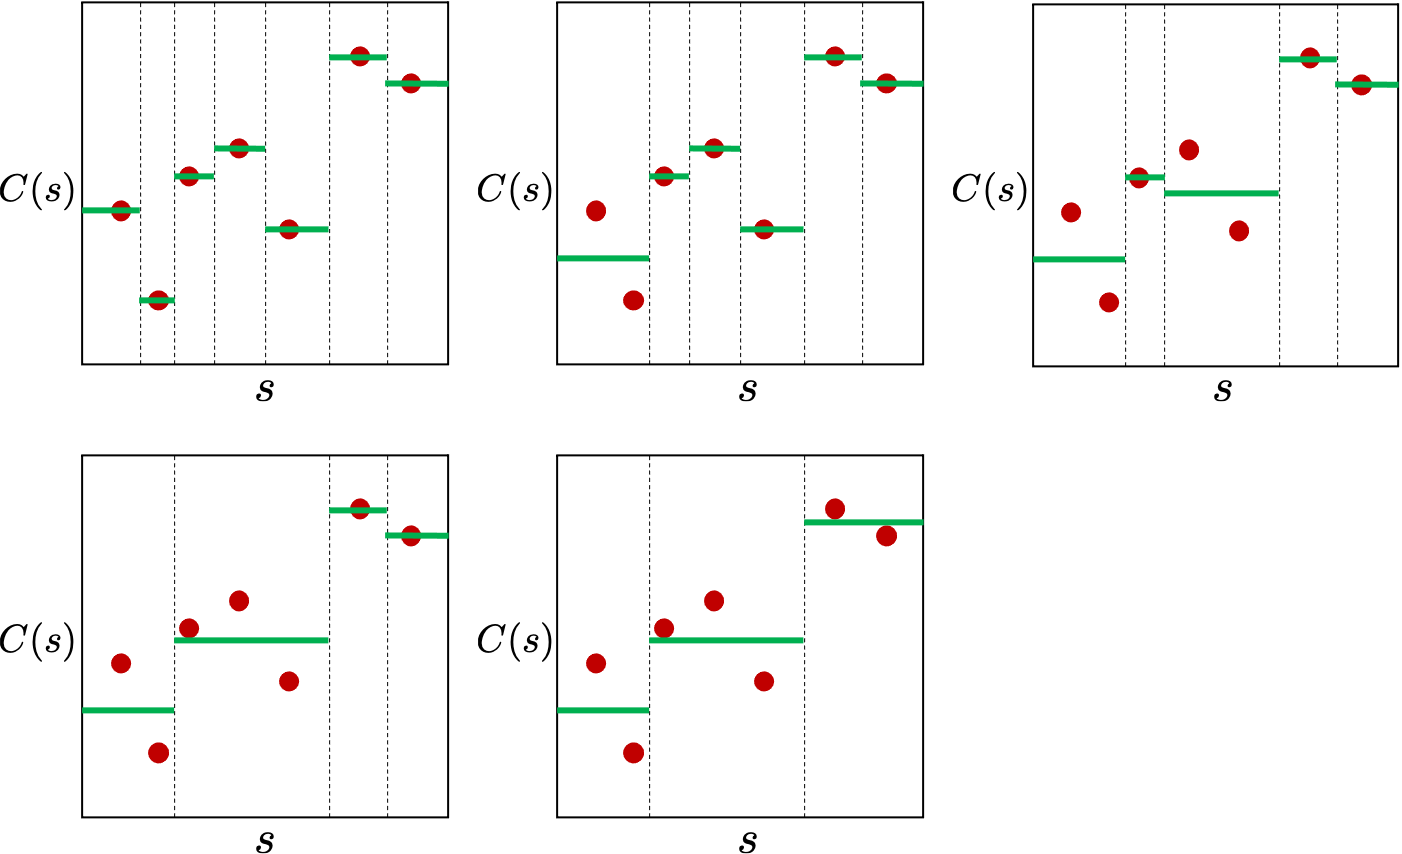
\includegraphics[width=0.9\textwidth]{figure/pic-pava}
		
% 	\end{center}
% \end{frame}

% \begin{frame}[t]
% 	\frametitle{Pair-adjacent violators algorithm (PAVA)}
	
% 	\begin{itemize}
% 		\item Note that, in the case of binary classification, the target values $y^{(n)}$ are all in $\{ 0, 1 \}$:
% 	\end{itemize}
	
% 	\medskip 
	
% 	\begin{center}
% 		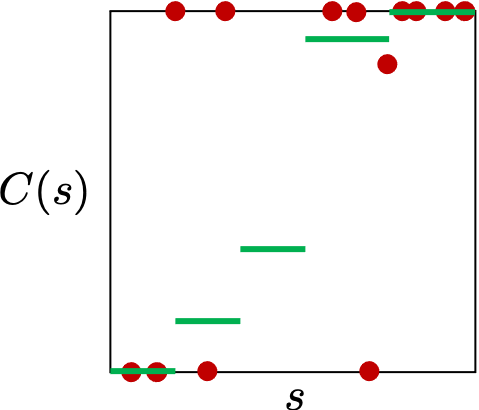
\includegraphics[width=0.4\textwidth]{figure/pic-pava2}
		
% 	\end{center}
% \end{frame}


\begin{frame}[t]
	\frametitle{Outlook: Multi-class calibration}
	
	\begin{itemize}
        \itemsep1em
		\item Calibration methods also exist for the multi-class case (i.e., classification problems with more than two classes).
		\item Then, however, the problem becomes conceptually more difficult (and is still a topic of ongoing research).
		\item 
		While essentially coinciding for binary classification, the following definitions of calibration (leading to increasingly difficult problems) can be distinguished for more than two classes:
		\begin{itemize}
			\item Calibration of the highest predicted probability (confidence calibration) 
			\item Calibration of the marginal probabilities (class-wise calibration)
			\item Calibration of the entire vector of predicted probabilities (multi-class calibration)
		\end{itemize}
        \item Recently, native multi-class calibration methods extended Platt scaling by adding a calibration layer between the logits of the neural network and the softmax layer. 
	\end{itemize}
\end{frame}





\begin{frame}{Why Is Calibration Important?}

    \begin{itemize}
        \item \textbf{Interpreting Predicted Probabilities:}
            \begin{itemize}
                \item They should accurately reflect actual risks or frequencies of events.
                \item Good calibration ensures that predicted probabilities match observed frequencies.
            \end{itemize}
            
        \item \textbf{Example: Medical Diagnosis}
            \begin{itemize}
                \item Well-calibrated models are crucial for informed decision-making.
                \item Poor calibration: Only half of patients with 90\% predicted probability of a disease actually have it.
                \item Good calibration: 90\% of patients with 90\% predicted probability of a disease actually have it.
                \item Poor calibration can lead to misdiagnosis, delayed or unnecessary treatment, affecting human lives.
            \end{itemize}
    \end{itemize}
\end{frame}

\endlecture
\end{document}
